




%%%%%%%%%%%%%%%%%%%%%%%%%%%%%%%%%%%%%%%%%%%%%%%%%%%%%%%%%%%%%%%%%%%%%%%%%%%%%%%%%%%%%%%%%%
\newpage
\chapter{Appendix}


%%%%%%%%%%%%%%%%%%%%%%%%%%%%%%%%%%%%%%%%%%%%%%%%%%%%%%%%%%%%%%%%%%%%%%%%%%%%%%%%%%%%%%%%%%%%%%%%%%%%%%%%%%%%%%%%%%%%%%
\section{Complex Number Quiz}\label{ComplexNumberQuiz}
Take this quiz then check your answers on Page \pageref{CN_answers}.  Use only the following functions on your calculator (or fewer as instructed):

\[
* \quad \div + \quad - \quad \sqrt{x}
\]


It should be {\bf easy for you to get exact answers}.  If not, then you need to review the concepts in this quiz and section \ref{cnconcepts}.   Some Kahn Academy videos are pre-linked in Section \ref{KahnV}.


\begin{enumerate}

\item  What is $\sqrt{-16}$ ?

\item  Evaluate
\[
X = \frac{-b + \sqrt{4ac}}{2a}
\]
for the following values:
\begin{quotation}
\begin{tabular} {c|c|c}
a&b&c  \\ \hline
1&2&3 \\
1&-4&29\\
2&28&1156
\end{tabular}
\end{quotation}


\item  Evaluate
\[
(6+j16) + (-7-j6) =
\]
\[
(27-j0.75) - (1.6+j0.27) =
\]


\item  Evaluate  $M\times N$ where

\begin{quotation}
\begin{tabular} {c|c}
M&N \\ \hline
$(2+6j)$	&	$(1+3j)$   	\\
$(1.7-0.6j)$    &	$(3.2+0.4j)$	\\
\end{tabular}
\end{quotation}


\item  Plot the following points on the complex plane:
\[
a = -3+1.5j \qquad b = 2-j \qquad c = j
\]


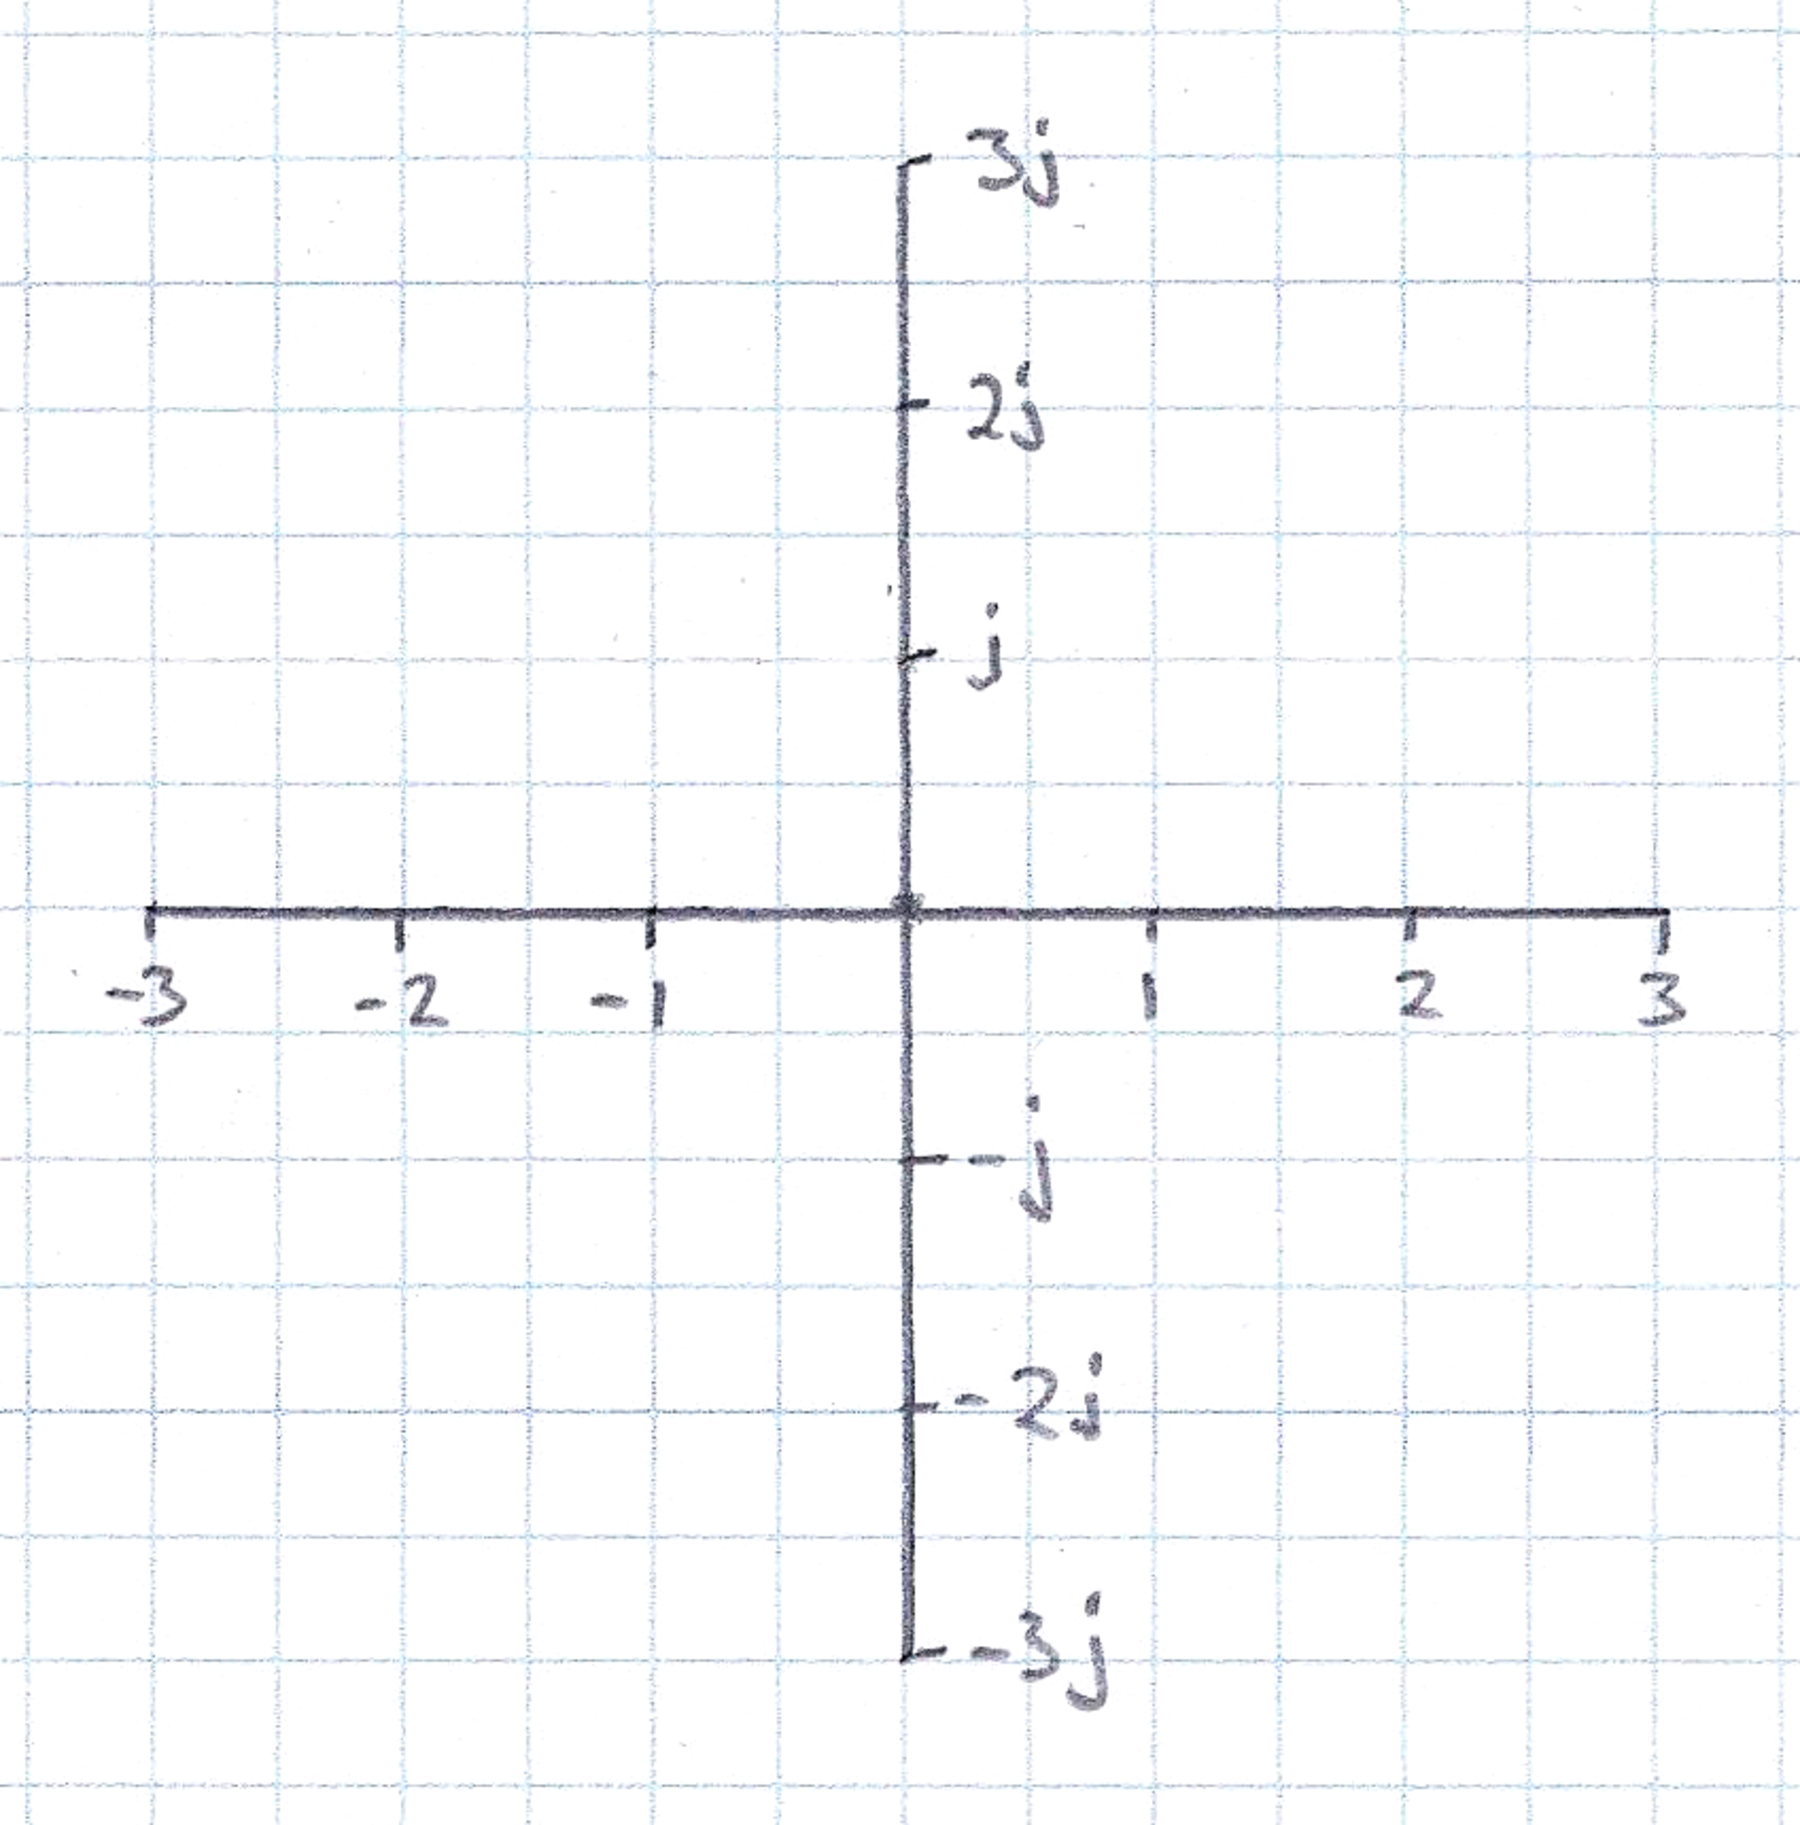
\includegraphics[width=6cm]{figsapdx/00926a.png}



\item  Convert $X_1=(4+3j)$ to polar (magnitude-angle) form


\item  Convert $X_2=(-16+3.7j)$ to polar (magnitude-angle) form


\item  Represent $X_3 = (-1+6j)$ in exponential form

\item  For
\[
a = 3e^{j\pi/4} \qquad b = 2\angle{45^\circ}
\]
Convert them to ``$a+bj$'' form and multiply $a*b$ without using a calculator.

\end{enumerate}




\clearpage
\newpage
\section{Complex Number Quiz Answers}\label{CN_answers}

\begin{enumerate}
\item 4j

\item $-1\pm j\sqrt{2} \qquad  2\pm j5 \qquad -7\pm j23  $

\item $-1+j10 \qquad 1.1-j1.02$

\item $-16+12j \qquad 5.68-1.24j$

\item graphing points $a,b,c$:

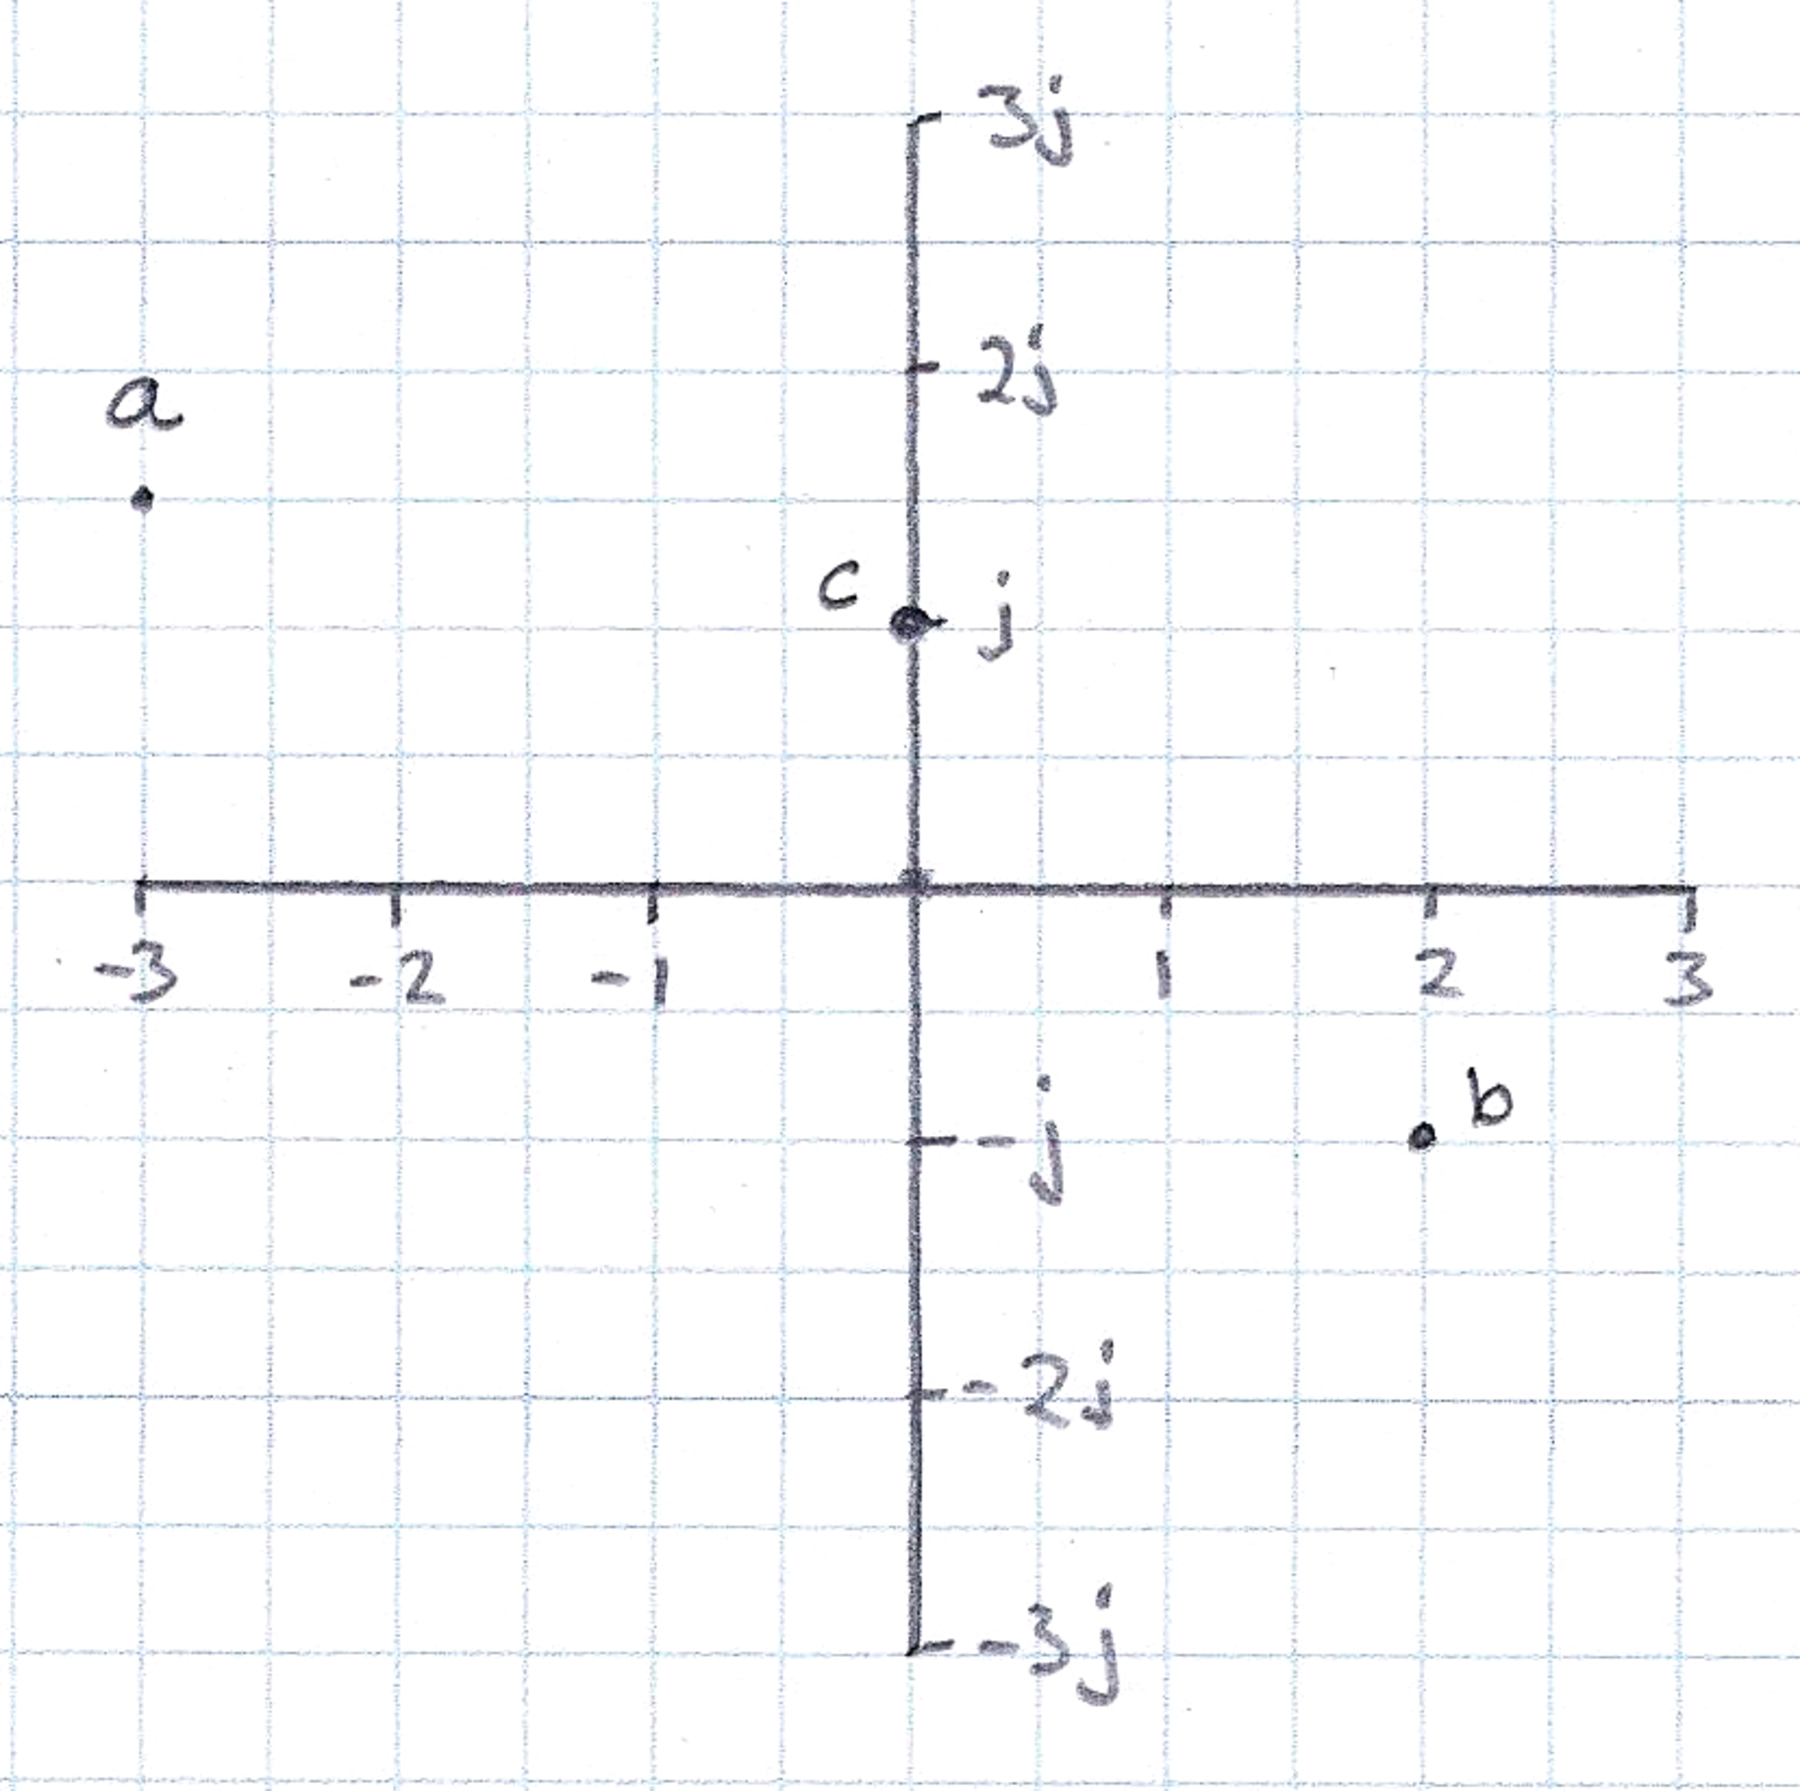
\includegraphics[width=6cm]{figsapdx/00927a.png}

\item $|X_1| = 5 \qquad \angle X_1 = \tan^{-1}(4/3) = 53.1^\circ$

\item $|X_2| = 16.42 \qquad \angle{X_2} = 167^\circ$

\item $X_3 = 6.08e^{j1.74}$ (note radians must be used in the exponential)

\item $|a| = 3, \; |b| = 2$,  $\angle a = 45^\circ,\; \angle b = 45^\circ$  by inspection.
\[
a = 3*0.707 + j3*0.707 = .2121+j.2121 \qquad b = 2*.707 + j2*.707 = .1414+j.1414
\]
using {\it angles add, magnitudes multiply}, $a*b = 3*2e^{j\frac{\pi}{2}} = 6e^j = 6j$

\end{enumerate}


%%%%%%%%%%%%%%%%%%%%%%%%%%%%%%%%%%%%%

\section{Log Quiz Answers}\label{Log_answers}


\begin{enumerate}

\item $\log(A) + \log(B)$

\item $2\log(a)+\frac{\log(b)}{2}$

\item $6-\log(R)$

\item $27.4$

\item $27.4/\ln(10)$

\end{enumerate}

